\section{ Messung von Amplituden- und Phasengang der Filterschaltungen }
In diesem Teil sollen die Amplituden und Phasengänge der Filter gemessen und aufgezeichnet werden.
Der hierfür verwendete Universalfilter wurde in der Vorbereitung analysiert.


\subsection*{Aufbau}
Der Universalfilter wird wie im Blockschaltbild an den Audioanalyzer angeschlossen.
Am Audioanalyzer wird das Program "AktFilt Ampl & Phase.set" gestartet und ausgeführt.

% grafik einbinden
\begin{figure}[H]
    \begin{center}
        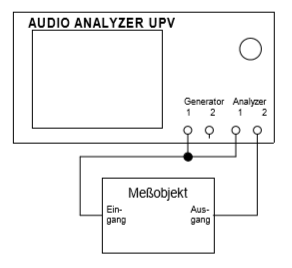
\includegraphics[width=0.5\textwidth]{img/Blockschalt.PNG}
        \caption{Blockschaltbild, Quelle: "GNP3 Aktive RC-Filter.pdf" }
        \label{fig:A3_label}
    \end{center}
\end{figure}






\subsection{Amplituden und Phasengängen von Butterworth-, Tschebyscheff- und Bessel-Tiefpass, logarithmischer}
Die Messung wird mit einem Frequenz "Sweep" von $\SI{100}{\hertz}-\SI{20}{\kilo\hertz}$ durchgeführt.
% grafik einbinden
\begin{figure}[H]
    \begin{center}
        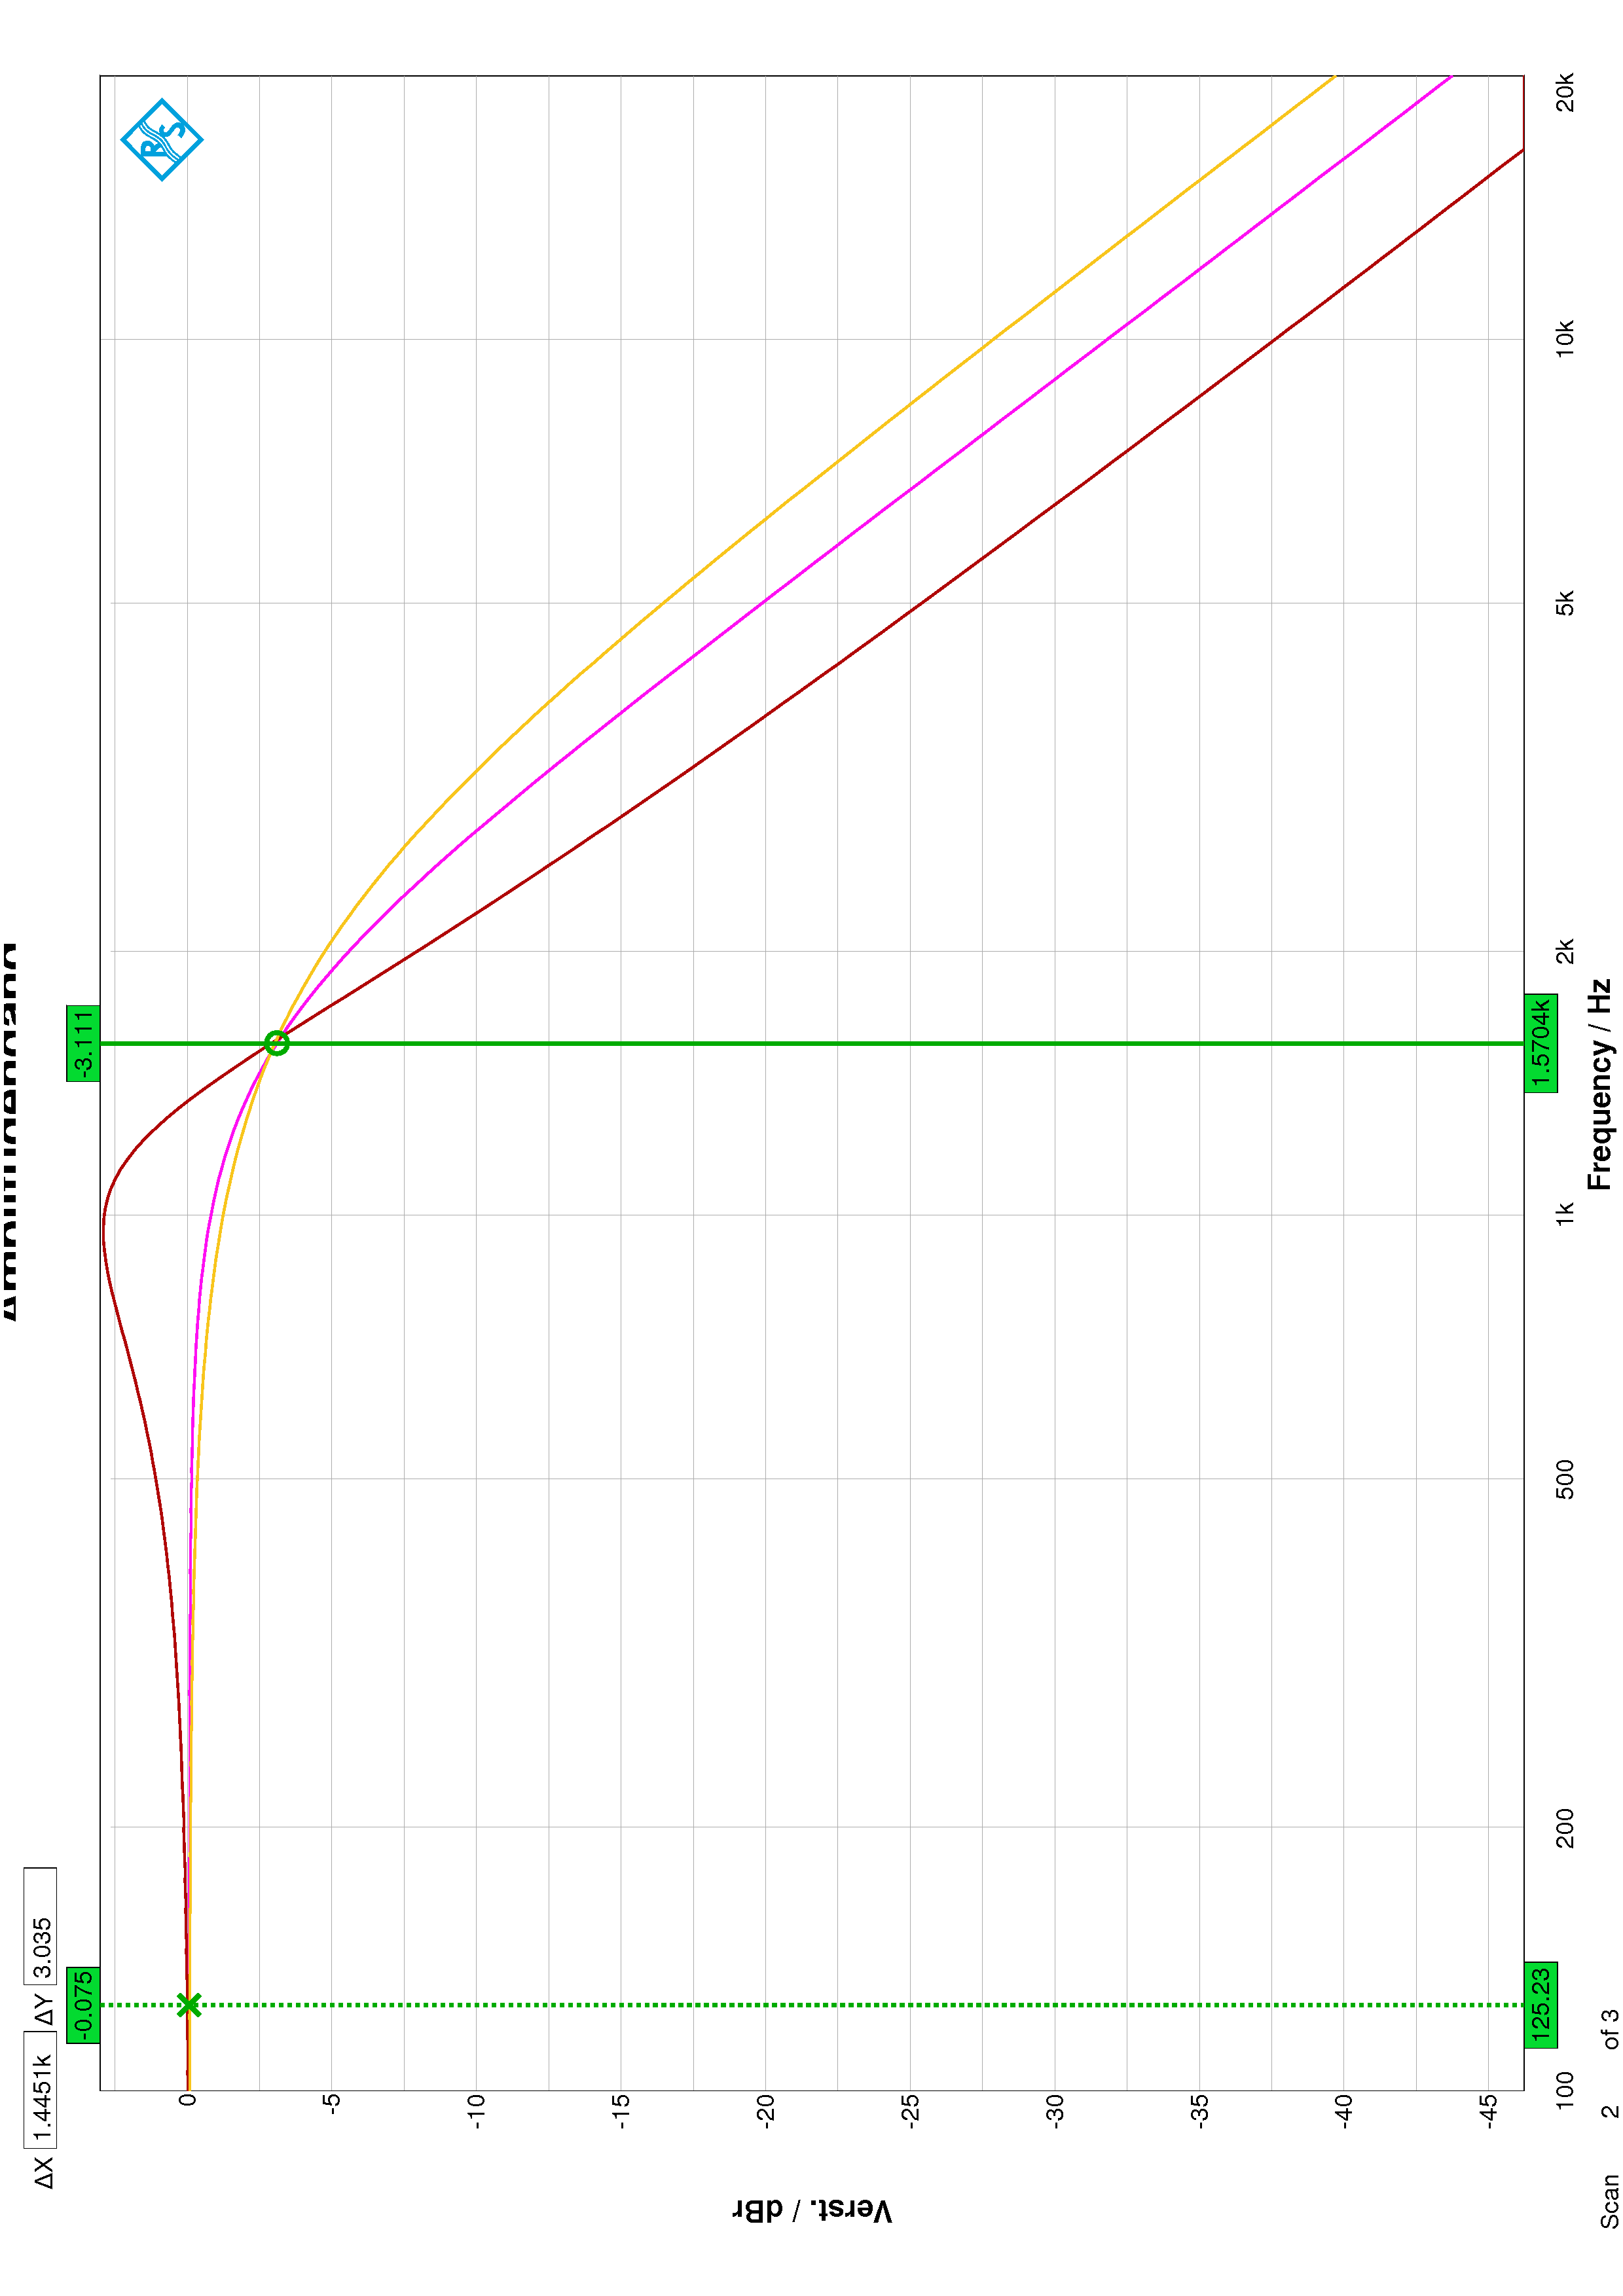
\includegraphics[width=0.8\textwidth, angle =-90]{img/3.1 Amplitudengang.png}
        \caption{Amplitudengang, Rot = Tschebyscheff, Pink = Butterworth , Gelb = Bessel}
        \label{fig:A3_amp}
    \end{center}
\end{figure}
Der Tschebyscheff filter  (Rote Linie) ist leicht an seinem deutlichem über schwingen kurz vor der Grenzfrequenz und schärfsten Abfall der Amplitude zu erkennen. Der Butterworth filter (Pinke Linie) ist der Filter der eine möglichst flache Kurve im Durchlassbereich aufweist. Bleibt noch der Bessel filter (Gelbe Linie) mit seinem geringem über schwingen.

% grafik einbinden
\begin{figure}[H]
    \begin{center}
        \includegraphics[width=0.8\textwidth, angle =-90]{img/3.1 Phasengänge.png} 
        \caption{Phasengänge, Rot = Tschebyscheff, Pink = Butterworth , Gelb = Bessel}
        \label{fig:A3_phase}
    \end{center}
\end{figure}

Aus den Messungen lassen sich die Grenzfrequenzen und Phasen der drei Filter ablesen:
\begin{table}[ht]
    \centering
    \begin{tabular}{|c|c|c|c|}\hline
    \tbf{Filter} & \tbf{Grenzfrequenz $f_g$} & \tbf{Phase $\SI{-60}{\degree}$}     &  \tbf{Phase $\SI{-120}{\degree}$}      \\ \hline
    Butterworth                   & \SI{1570.4}{\hertz} &     \SI{1069.2}{} &\SI{2417.2}{}     \\
    Tschebyscheff             & \SI{1582.6}{\hertz}  &   \SI{915.3}{}  &\SI{1425.2}{}    \\ 
    Bessel                &\SI{1582.6}{\hertz}   &\SI{1248.9}{}&\SI{3298.2}{}  \\ \hline
    \end{tabular}
    \caption{Filter Parameter}
\end{table}




\subsection{Phasengänge von Butterworth-, Tschebyscheff- und Bessel-Tiefpass gemeinsam in einem Plot über linearer Frequenzachse, Frequenzbereich 100Hz...4kHz. }


\begin{table}[ht]
    \centering
    \begin{tabular}{|c|c|c|c|}\hline
    \tbf{Filter} & \tbf{Grenzfrequenz $f_g$} & \tbf{Phase $\SI{-60}{\degree}$}     &  \tbf{Phase $\SI{-120}{\degree}$}     \\ \hline
    Butterworth                   & \SI{1584.6}{\hertz} &     \SI{1251.3}{} &\SI{3283.9}{}     \\
    Tschebyscheff             & \SI{1578.9}{\hertz}  &   \SI{914.6}{}  &\SI{1419.8}{}    \\ 
    Bessel                &\SI{1584.6}{\hertz}   &\SI{1066.4}{}&\SI{2404.5}{}  \\ \hline
    \end{tabular}
    \caption{Grenzfrequenzen der Filter}
\end{table}

% grafik einbinden
\begin{figure}[H]
    \begin{center}
        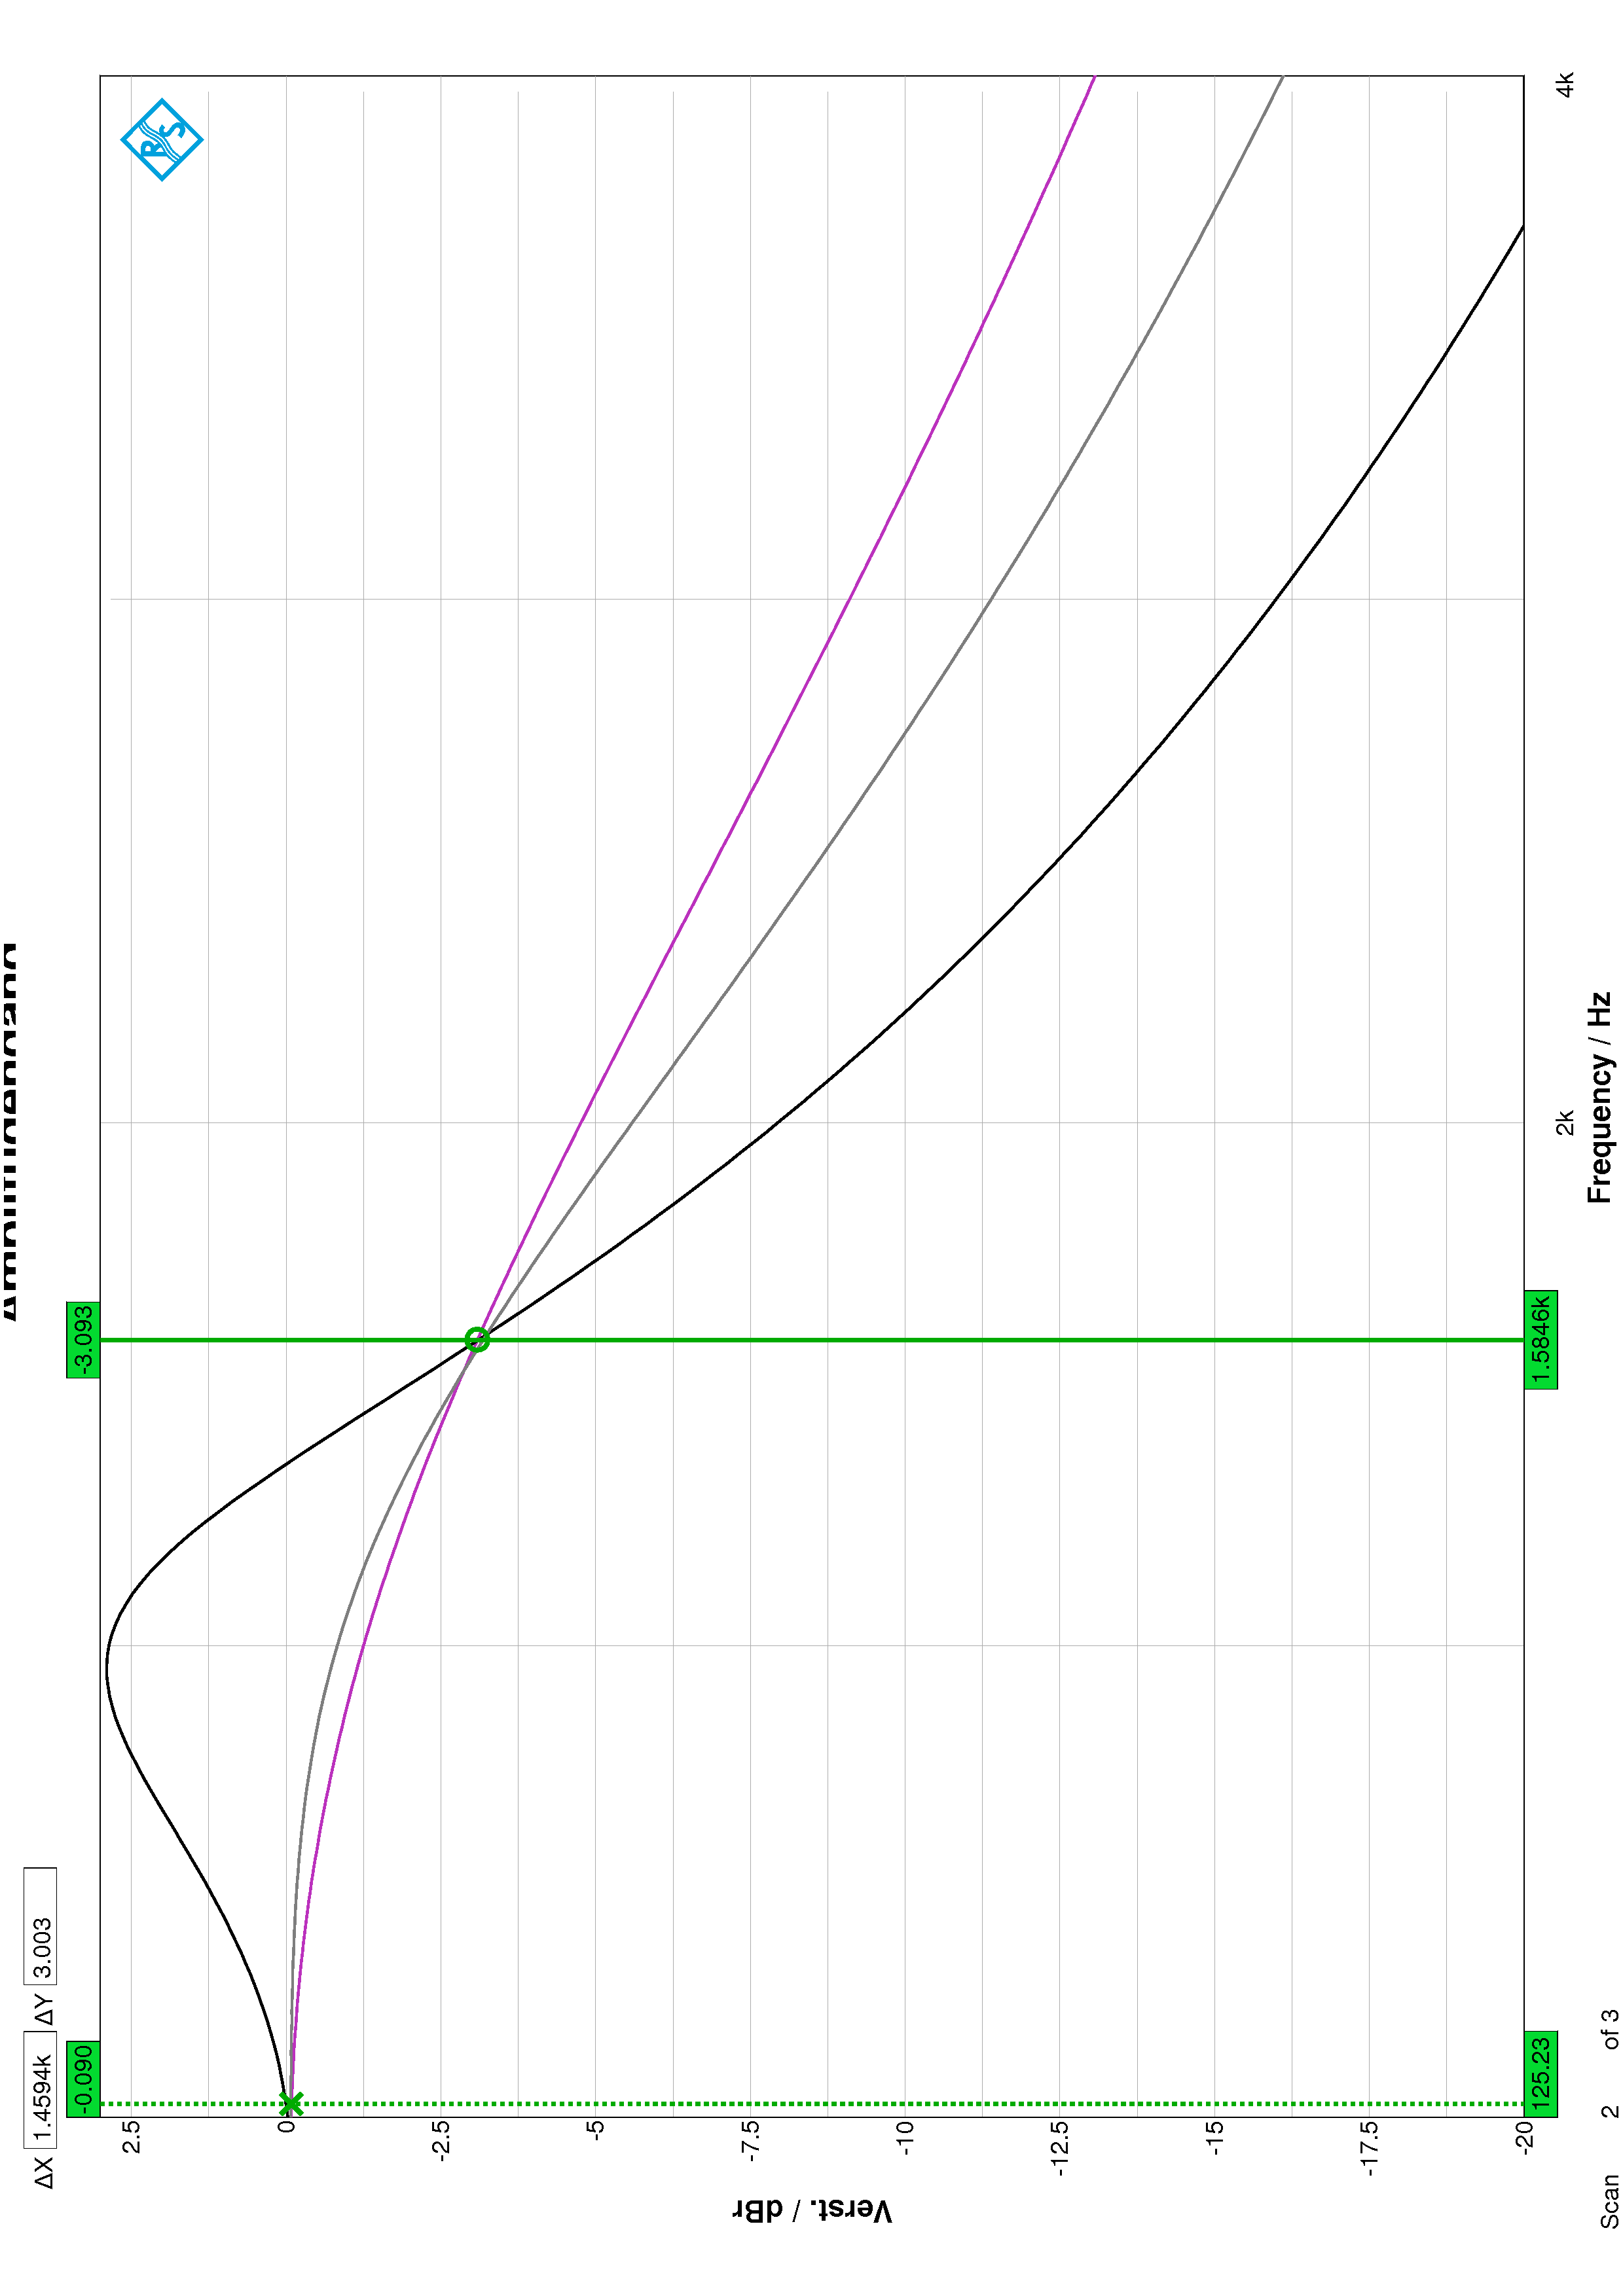
\includegraphics[width=0.8\textwidth, angle =-90]{img/3.2 Amplitudengang linear.png}
        \caption{Amplitudengang linear}
        \label{fig:A3_amp}
    \end{center}
\end{figure}
+

% grafik einbinden
\begin{figure}[H]
    \begin{center}
        \includegraphics[width=0.8\textwidth, angle =-90]{img/3.2 Phasengänge linear.png}
        \caption{Phasengänge linear}
        \label{fig:A3_phase}
    \end{center}
\end{figure}






\subsection{Amplitudengänge (mit Phasengängen) von Butterworth-, Tschebyscheff- und BesselHochpass gemeinsam in einem Plot über logarithmischer Frequenzachse, Frequenzbereich 100Hz...20kHz. }


\begin{table}[ht]
    \centering
    \begin{tabular}{|c|c|c|c|}\hline
    \tbf{Filter}     & \tbf{Grenzfrequenz $f_g$}  \\ \hline
    Butterworth                   & \SI{1632.5}{\hertz}            \\
    Tschebyscheff             & \SI{1607.3}{\hertz}           \\ 
    Bessel                &\SI{1619.8}{\hertz}     \\ \hline
    \end{tabular}
    \caption{Grenzfrequenzen der Filter}
\end{table}

% grafik einbinden
\begin{figure}[H]
    \begin{center}
        \includegraphics[width=0.8\textwidth, angle =-90]{img/3.3 Amplitudengänge HP log.png}
        \caption{\imgfilename}
        \label{fig:A3b_label}
    \end{center}
\end{figure}

% grafik einbinden
\begin{figure}[H]
    \begin{center}
        \includegraphics[width=0.8\textwidth, angle =-90]{img/3.3 Phasengänge HP log.png}
        \caption{\imgfilename}
        \label{fig:A3c_label}
    \end{center}
\end{figure}





\subsection{Amplitudengänge (mit Phasengängen) von Bandpass und Bandsperre gemeinsam in einem Plot über logarithmischer Frequenzachse, Frequenzbereich 1kHz...2,5kHz. }
 

%multi figure
\begin{figure}[H]
\begin{center}
\subfloat[Amplitudengang Bandpass]{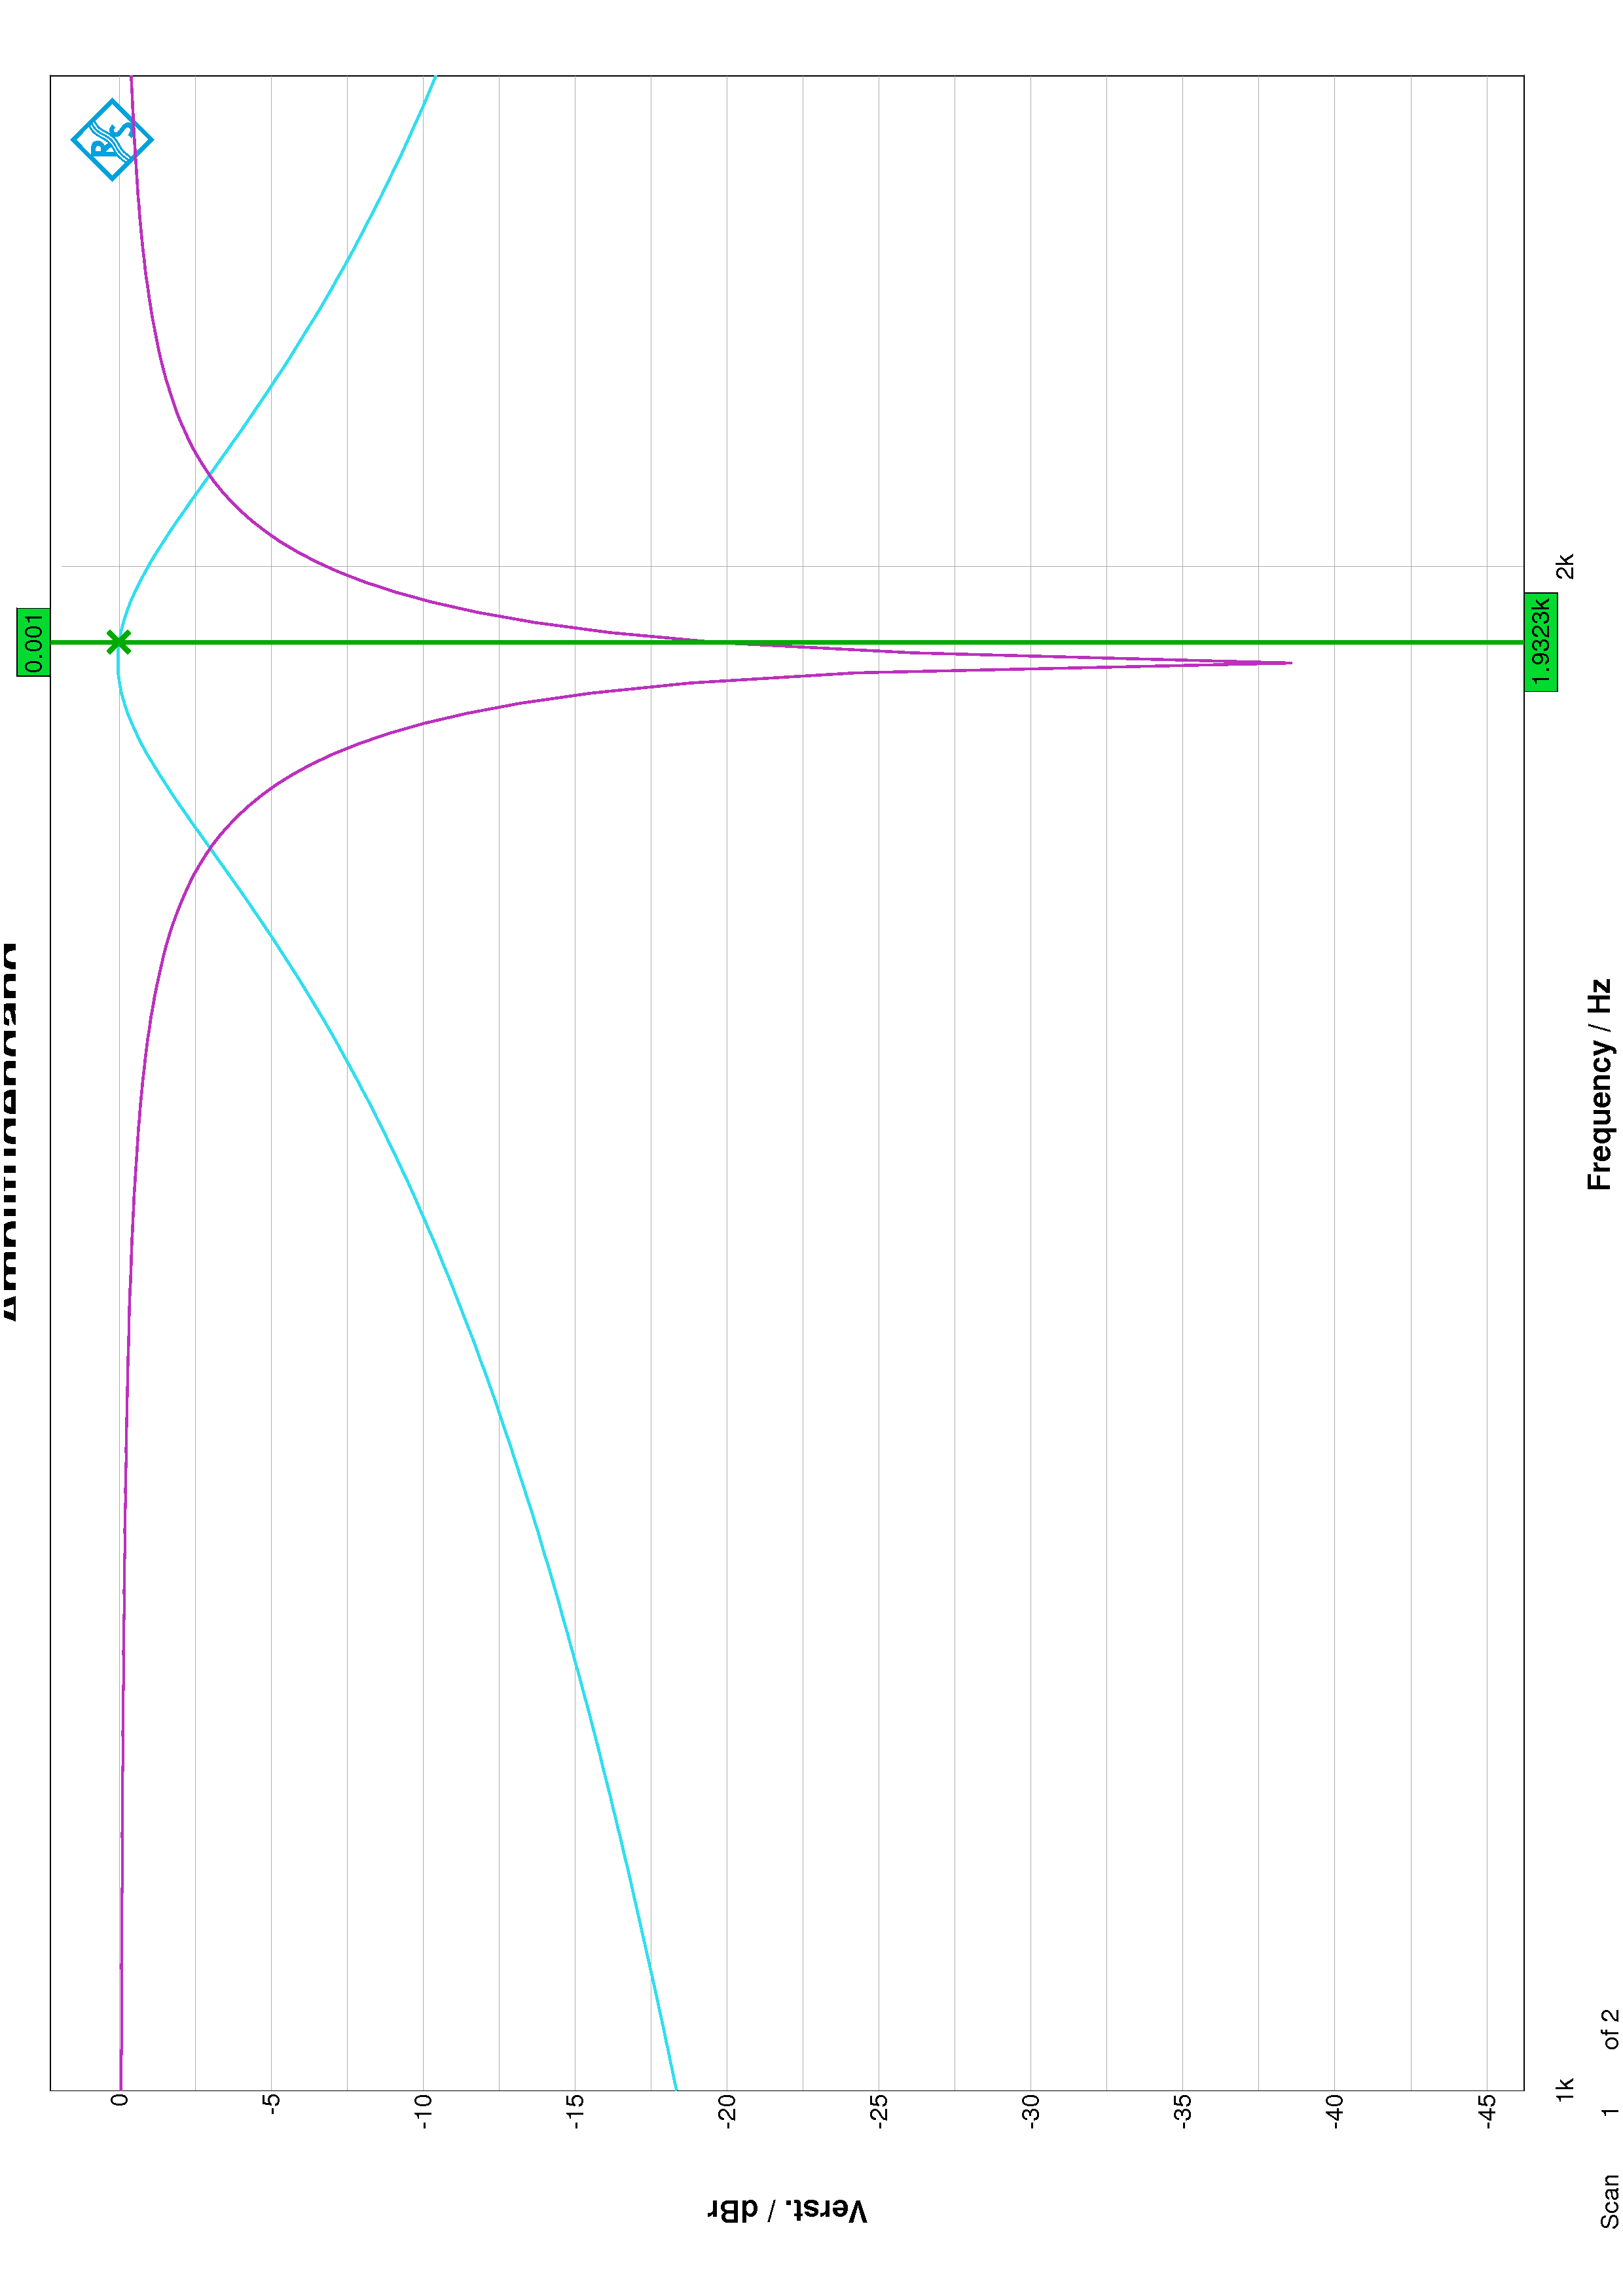
\includegraphics[width = \textwidth/3, angle =-90]{img/3.4 Amplitudengang Bandpass.png}}  
\subfloat[Amplitudengang Bandsperre]{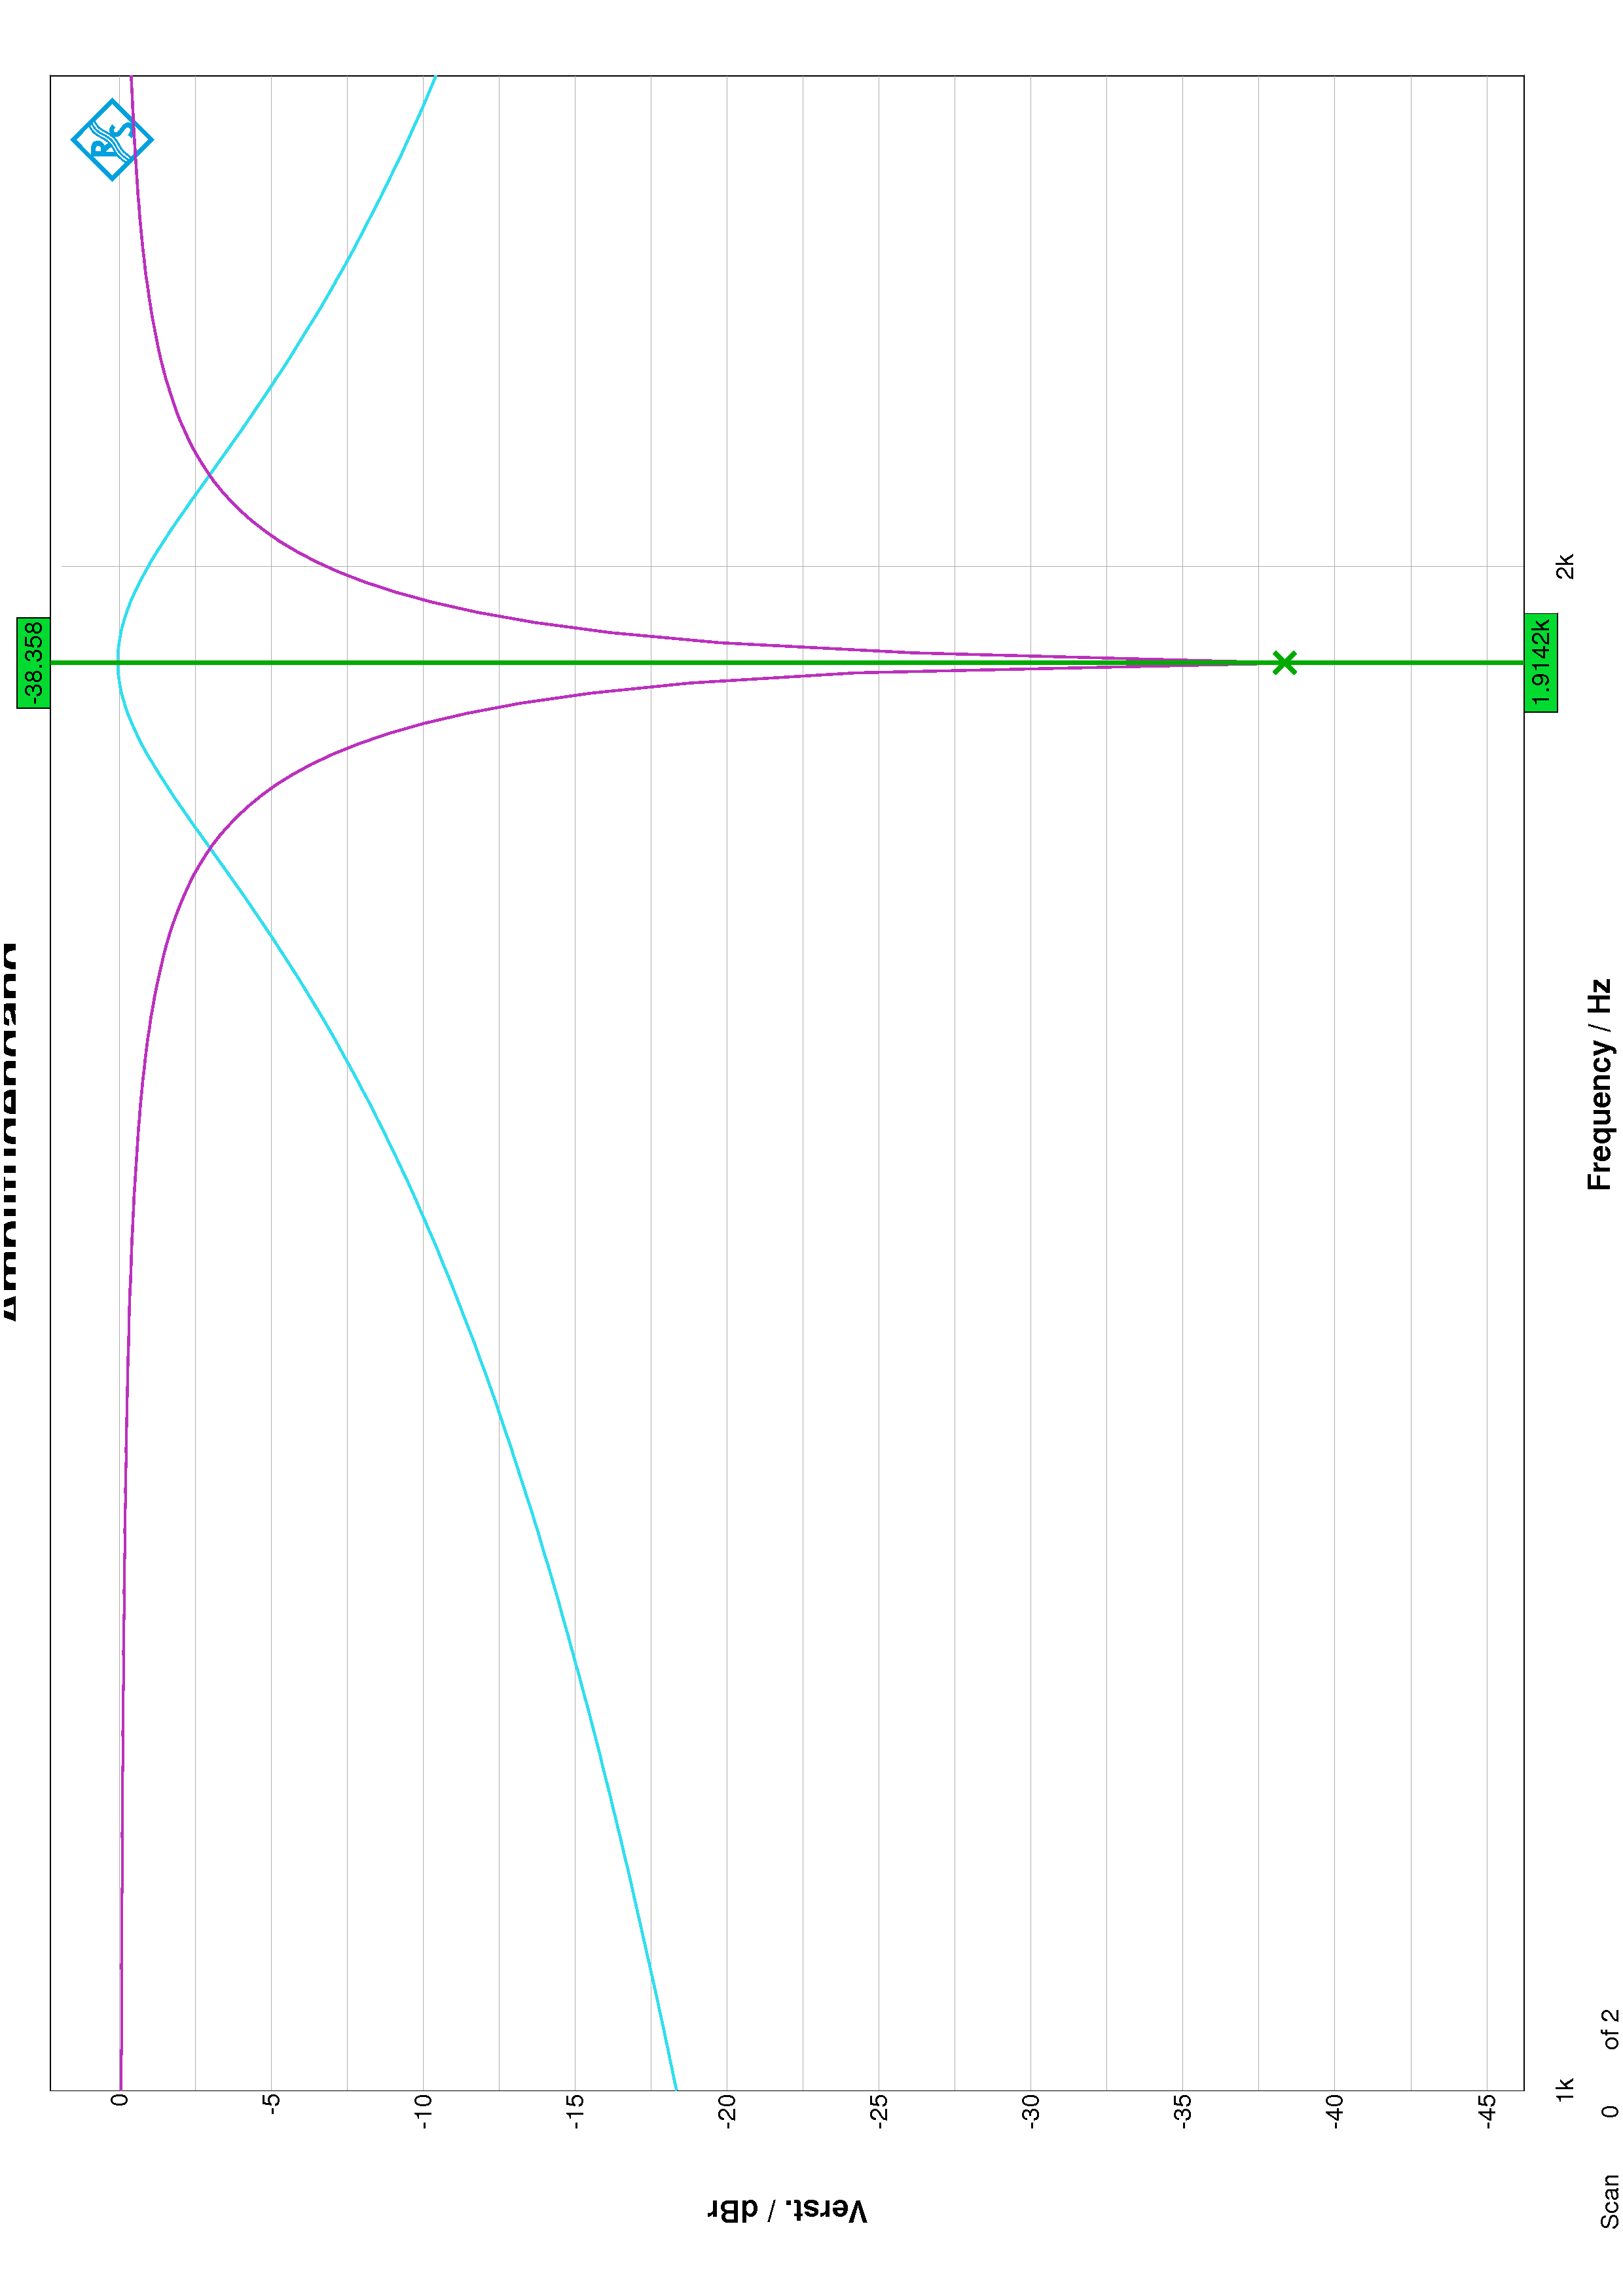
\includegraphics[width = \textwidth/3, angle =-90]{img/3.4 Amplitudengang Bandsperre.png}}\\
\subfloat[Bandbreite Bandpass]{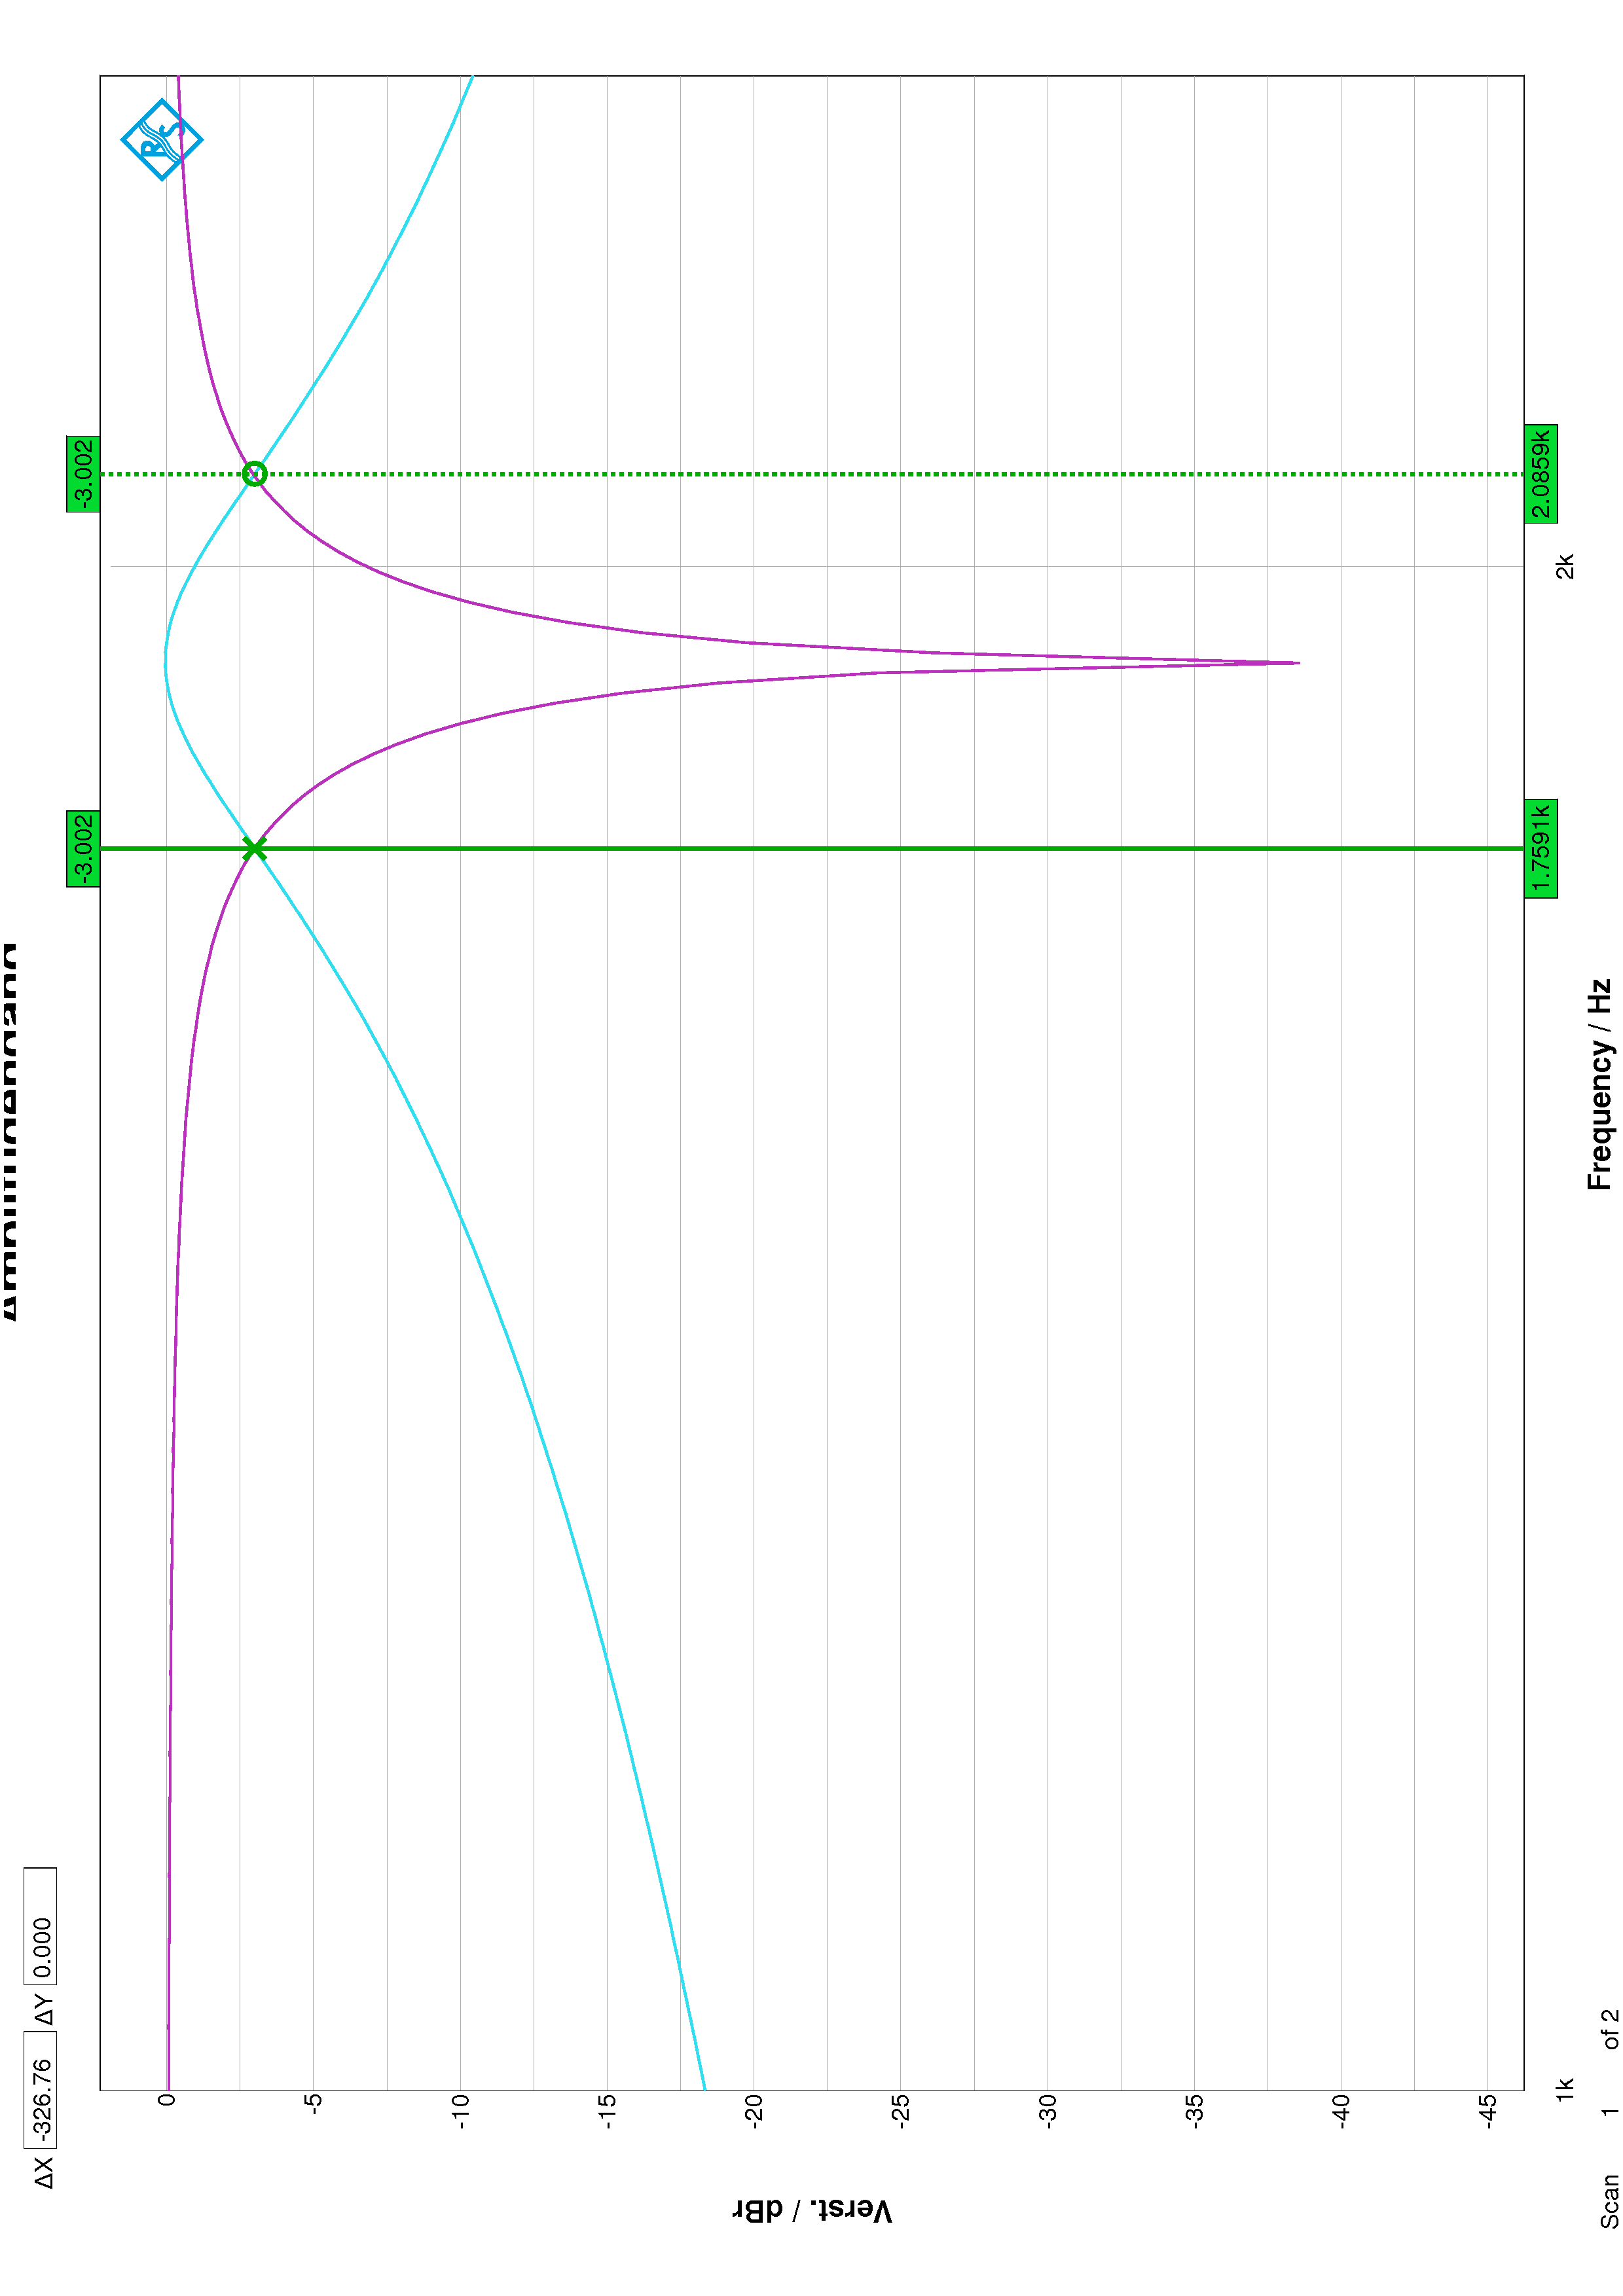
\includegraphics[width = \textwidth/3, angle =-90]{img/3.4 Bandbreite Bandpass.png}} 
\subfloat[Bandbreite Bandsperre]{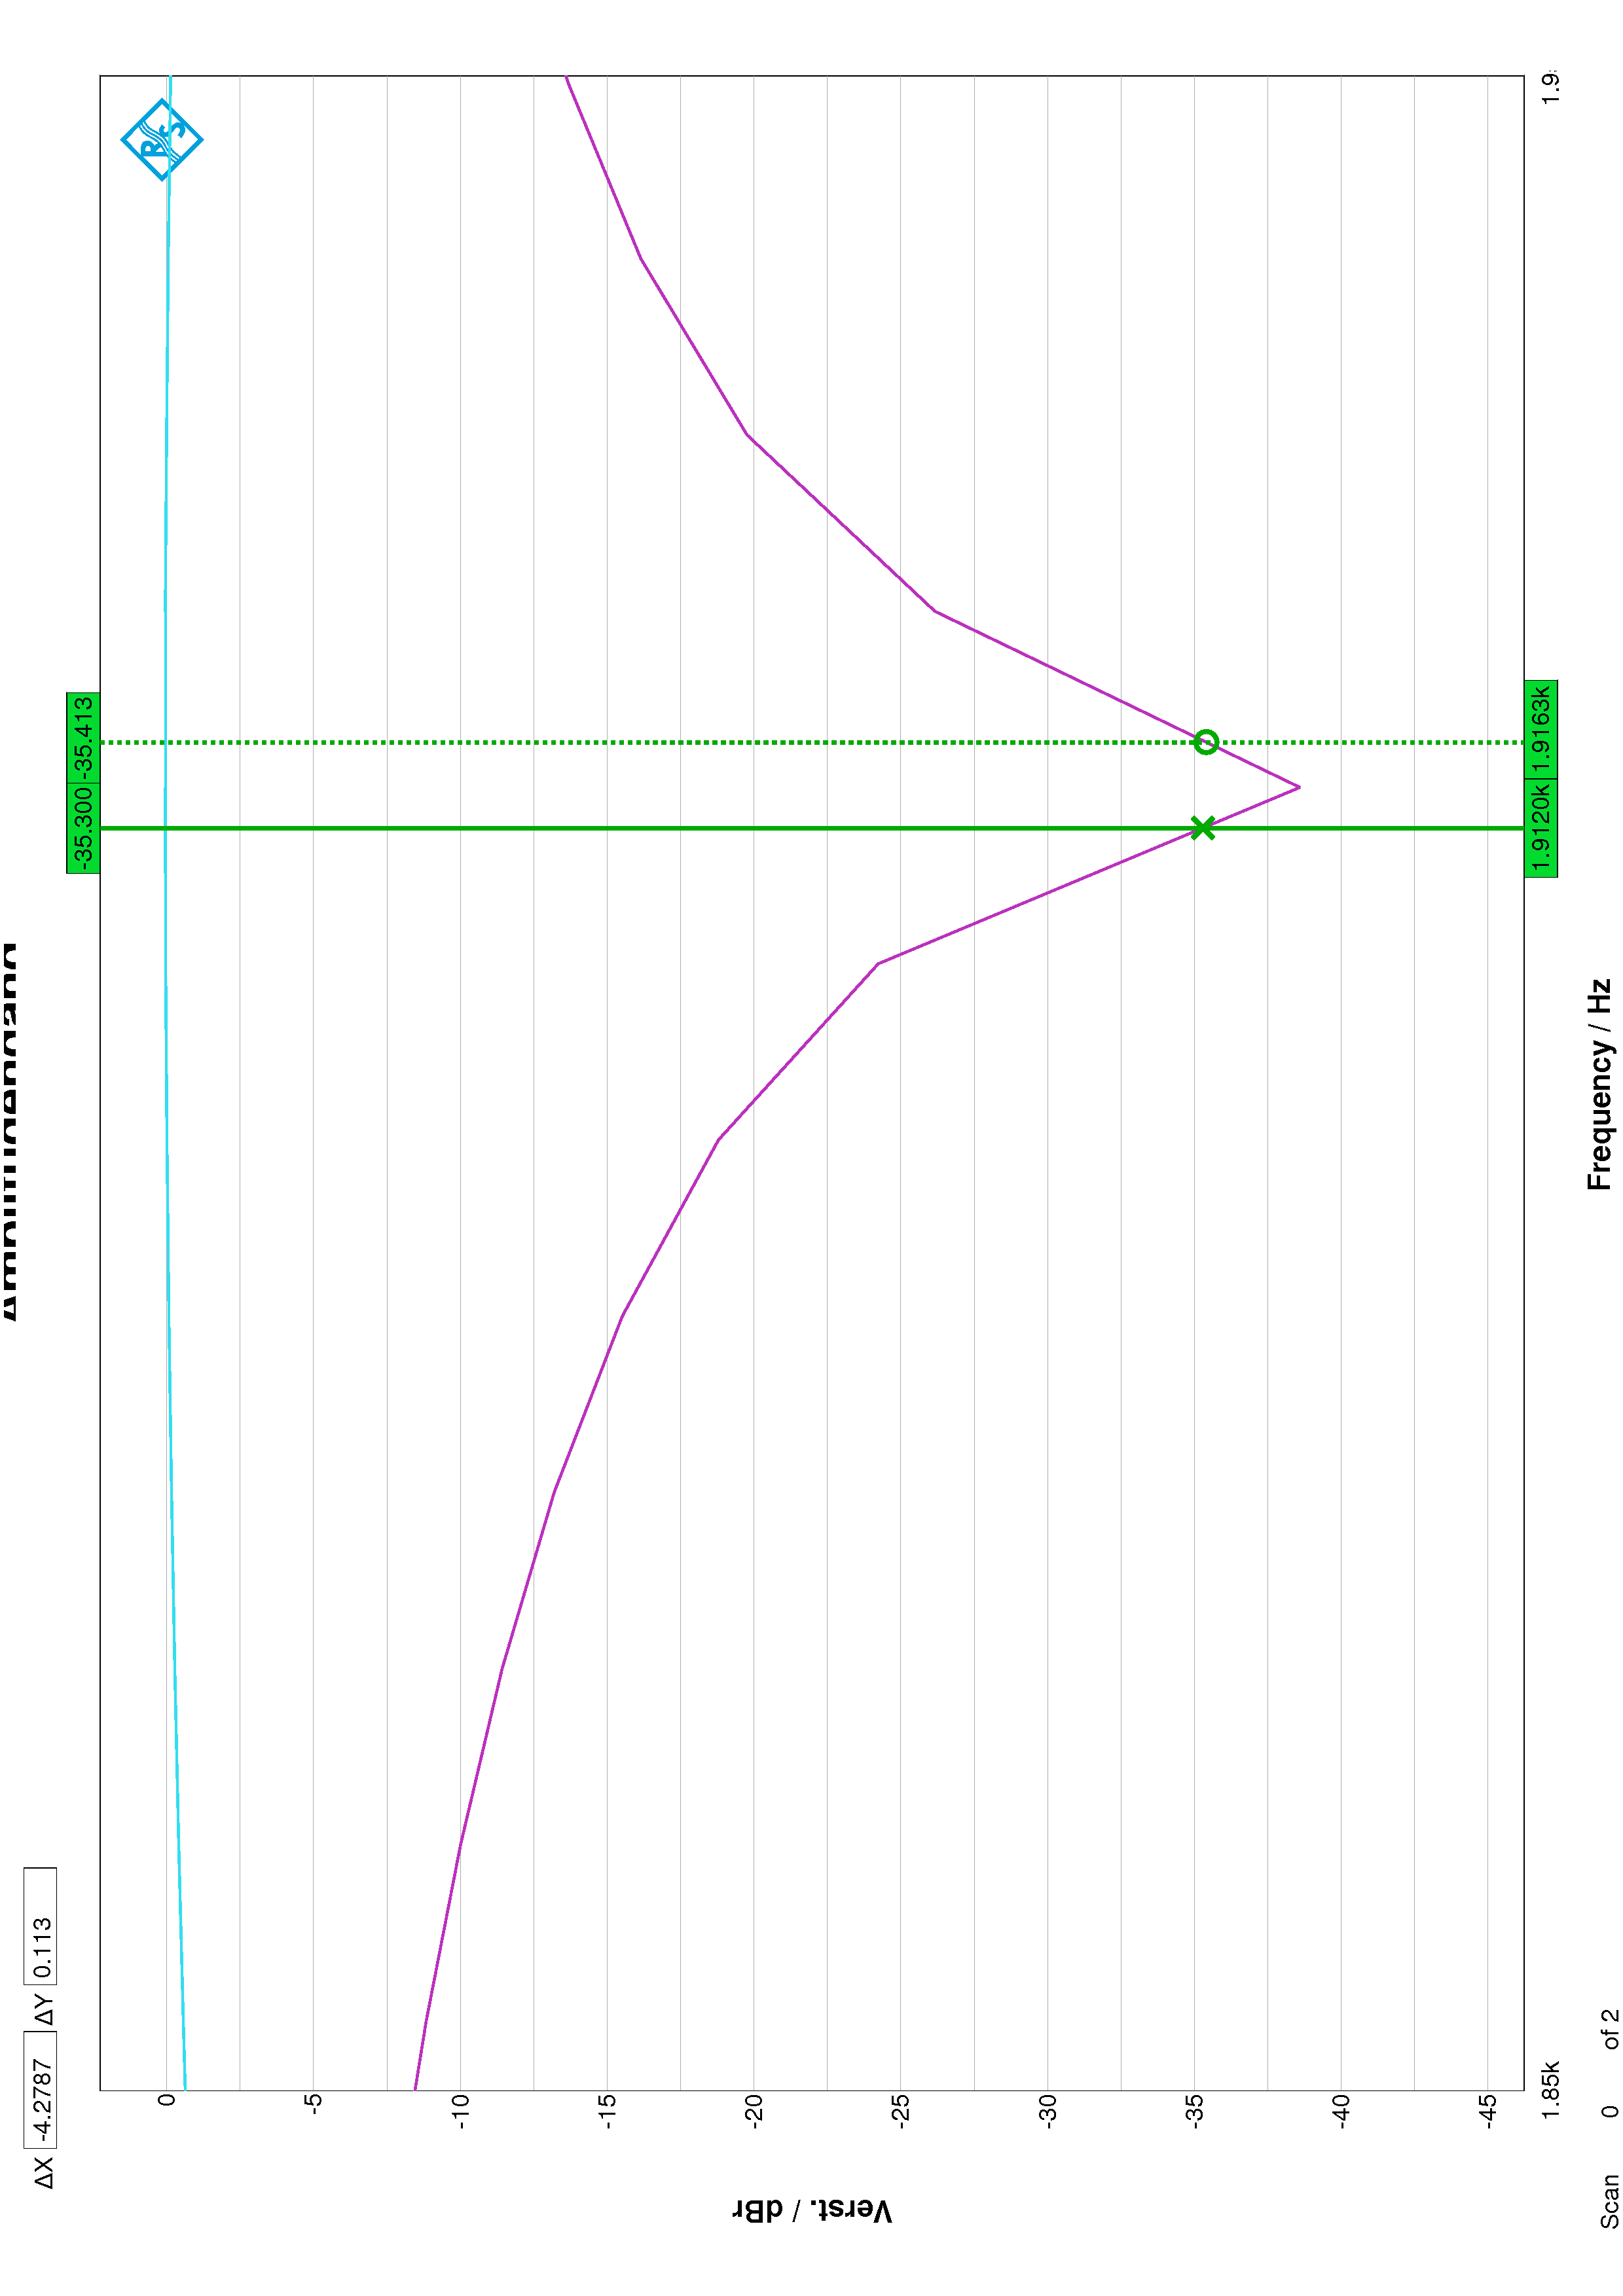
\includegraphics[width = \textwidth/3, angle =-90]{img/3.4 Bandbreite Bandsperre.png}} 
\caption{Bandbreiten}
\label{fig:A3_mult}
\end{center}
\end{figure}


\begin{table}[ht]
    \centering
    \begin{tabular}{|c|c|c|c|}\hline
    \tbf{Filter}     & \tbf{Mitte} & \tbf{$\SI{-3}{\decibel}$ unten} & \tbf{$\SI{-3}{\decibel}$ oben} \\ \hline
    Bandpass                   & \SI{1932.3}{\hertz}  & \SI{1759.1}{\hertz} & \SI{2085.9}{\hertz}\\
    Bandsperre                 & \SI{1914.2}{\hertz}  & \SI{1912}{\hertz} & \SI{1916.3}{\hertz}\\ \hline
    \end{tabular}
    \caption{Beispiel Addieren:}
\end{table}






%Amplitudengänge von Butterworth-, Tschebyscheff- und Bessel-Tiefpass und Markierung der Grenzfrequenzen Phasengänge von Butterworth-, Tschebyscheff- und Bessel-Tiefpass und Markierung der Frequenzen für eine Phasenverschiebung von -60° und -120° Amplitudengänge von Butterworth-, Tschebyscheff- und Bessel-Hochpass und Markierung der Grenzfrequenzen Amplitudengänge von Bandpass und Bandsperre und Markierung der Grenzfrequenzen Auswertung: Alle Messwerte der Grenzfrequenzen sind in einer Tabelle mit den Vorgabewerten einzutragen und zu vergleichen; Aus den Frequenzen bei 60° und 120° Phasenverschiebung sind die Koeffizienten a1, b1 der 3 Tiefpässe zu berechnen und mit den Vorgabewerten zu vergleichen 





















\subsection{Auswertung}
%%%%%%%%%%%%%%%%%%%%%%%%%%%%%%%%%%%%%%%%%%%%%%%%Comments
%Amplitudengänge von Butterworth-, Tschebyscheff- und Bessel-Tiefpass und Markierung der Grenzfrequenzen Phasengänge von Butterworth-, Tschebyscheff- und Bessel-Tiefpass und Markierung der Frequenzen für eine Phasenverschiebung von -60° und -120° Amplitudengänge von Butterworth-, Tschebyscheff- und Bessel-Hochpass und Markierung der Grenzfrequenzen Amplitudengänge von Bandpass und Bandsperre und Markierung der Grenzfrequenzen Auswertung: Alle Messwerte der Grenzfrequenzen sind in einer Tabelle mit den Vorgabewerten einzutragen und zu vergleichen; Aus den Frequenzen bei 60° und 120° Phasenverschiebung sind die Koeffizienten a1, b1 der 3 Tiefpässe zu berechnen und mit den Vorgabewerten zu vergleichen